%% MODELO DE LATEX PARA TRABALHOS ACADÊMICOS
%% INSTRUÇÕES GERAIS:
%%    1. TODO O TEXTO NA FRENTE DO SIMBOLO '%' É COMENTÁRIO, ISTO É, ELE NÃO FAZ DIFERENÇA NO RESULTADO FINAL 
%%    2. NESTE MODELO, VOCÊS SÓ PRECISAM EDITAR DAS LINHAS 114 A 132 (INFORMAÇÕES DE CAPA) E DAS LINHAS 188 EM DIANTE (CORPO DO TRABALHO). O RESTO SÃO CONFIGURAÇÕES DE FORMATAÇÃO QUE PROVAVELMENTE NÃO SERÁ PRECISO MODIFICAR.
%%    3. MAIS INSTRUÇÕES DETALHADAS PODERÃO SER ENCONTRADAS NA PÁGINA profhelioh.wordpress.com. DÚVIDAS: heliohenrique@ufpr.br OU heliohenrique3@gmail.com

% INFORMAÇÕES DA FONTE:
%% abtex2-modelo-relatorio-tecnico.tex, v-1.7.1 laurocesar
%% Copyright 2012-2013 by abnTeX2 group at http://abntex2.googlecode.com/ 
%%
%% This work may be distributed and/or modified under the
%% conditions of the LaTeX Project Public License, either version 1.3
%% of this license or (at your option) any later version.
%% The latest version of this license is in
%%   http://www.latex-project.org/lppl.txt
%% and version 1.3 or later is part of all distributions of LaTeX
%% version 2005/12/01 or later.
%%
%% This work has the LPPL maintenance status `maintained'.
%% 
%% The Current Maintainer of this work is the abnTeX2 team, led
%% by Lauro César Araujo. Further information are available on 
%% http://abntex2.googlecode.com/
%%
%% This work consists of the files abntex2-modelo-relatorio-tecnico.tex,
%% abntex2-modelo-include-comandos and abntex2-modelo-references.bib
%%
% ------------------------------------------------------------------------
% ------------------------------------------------------------------------
% abnTeX2: Modelo de Relatório Técnico/Acadêmico em conformidade com 
% ABNT NBR 10719:2011 Informação e documentação - Relatório técnico e/ou
% científico - Apresentação
% ------------------------------------------------------------------------ 
% ------------------------------------------------------------------------

\documentclass[
	% -- opções da classe memoir --
	12pt,				% tamanho da fonte
	% openright,			% capítulos começam em pág ímpar (insere página vazia caso preciso)
    oneside,			% para impressão somente frente. Oposto a twoside (frente e verso)
	a4paper,			% tamanho do papel. 
	% -- opções da classe abntex2 --
	%chapter=TITLE,		% títulos de capítulos convertidos em letras maiúsculas
	%section=TITLE,		% títulos de seções convertidos em letras maiúsculas
	%subsection=TITLE,	% títulos de subseções convertidos em letras maiúsculas
	%subsubsection=TITLE,% títulos de subsubseções convertidos em letras maiúsculas
	% -- opções do pacote babel --
	english,			% idioma adicional para hifenização
	french,				% idioma adicional para hifenização
	spanish,			% idioma adicional para hifenização
	brazil,				% o último idioma é o principal do documento
	]{abntex2}


% ---
% PACOTES
% ---

% ---
% Pacotes fundamentais 
% ---
\usepackage{cmap}				% Mapear caracteres especiais no PDF
\usepackage{lmodern}			% Usa a fonte Latin Modern
\usepackage[T1]{fontenc}		% Selecao de codigos de fonte.
\usepackage[utf8]{inputenc}		% Codificacao do documento (conversão automática dos acentos)
\usepackage{indentfirst}		% Indenta o primeiro parágrafo de cada seção.
\usepackage{color}				% Controle das cores
\usepackage{graphicx}			% Inclusão de gráficos
% ---

% ---
% Pacotes adicionais, usados no anexo do modelo de folha de identificação
% ---
\usepackage{multicol}
\usepackage{multirow}
% ---
	
% ---
% Pacotes adicionais, usados apenas no âmbito do Modelo Canônico do abnteX2
% ---
\usepackage{lipsum}				% para geração de dummy text
% ---

% ---
% Pacotes de citações
% ---
\usepackage[brazilian,hyperpageref]{backref}	 % Paginas com as citações na bibl
\usepackage[alf]{abntex2cite}	% Citações padrão ABNT

% --- 
% CONFIGURAÇÕES DE PACOTES
% --- 

% ---
% Configurações do pacote backref
% Usado sem a opção hyperpageref de backref
\renewcommand{\backrefpagesname}{Citado na(s) página(s):~}
% Texto padrão antes do número das páginas
\renewcommand{\backref}{}
% Define os textos da citação
\renewcommand*{\backrefalt}[4]{
	\ifcase #1 %
		Nenhuma citação no texto.%
	\or
		Citado na página #2.%
	\else
		Citado #1 vezes nas páginas #2.%
	\fi}%
% ---

% ---
% Informações de dados para CAPA e FOLHA DE ROSTO
% ---
\titulo{Apresentação de Proposta: Abordagem Genérica ppara Sistemas de Recomendações}
\autor{Guilherme Müller Moreira}
\orientador{Marco André Abud Kappel}
\coorientador{Luis Claudio Batista da Silva}
\local{Brasil}
\data{13 de novembro de 2018}
\instituicao{%
  Centro de Ensino Técnico Federal Celso Suckow da Fonseca
  \par
  Uned Nova Friburgo
  \par
  Sistemas de Informação}
\tipotrabalho{Relatório técnico}
% O preambulo deve conter o tipo do trabalho, o objetivo, 
% o nome da instituição e a área de concentração 
\preambulo{Apresentação da proposta de projeto para trabalho de conclusão do curso de Sistemas de Informação do CEFET Nova Friburgo. O projeto propõe uma abordagem genérica para sitemas de recomendação.}
% ---

% ---
% Configurações de aparência do PDF final

% alterando o aspecto da cor azul
\definecolor{blue}{RGB}{41,5,195}

% informações do PDF
\makeatletter
\hypersetup{
     	%pagebackref=true,
		pdftitle={\@title}, 
		pdfauthor={\@author},
    	pdfsubject={\imprimirpreambulo},
	    pdfcreator={LaTeX with abnTeX2},
		pdfkeywords={abnt}{latex}{abntex}{abntex2}{relatório técnico}, 
		colorlinks=true,       		% false: boxed links; true: colored links
    	linkcolor=blue,          	% color of internal links
    	citecolor=blue,        		% color of links to bibliography
    	filecolor=magenta,      		% color of file links
		urlcolor=blue,
		bookmarksdepth=4
}
\makeatother
% --- 

% --- 
% Espaçamentos entre linhas e parágrafos 
% --- 

% O tamanho do parágrafo é dado por:
\setlength{\parindent}{1.3cm}

% Controle do espaçamento entre um parágrafo e outro:
\setlength{\parskip}{0.2cm}  % tente também \onelineskip

% ---
% compila o indice
% ---
\makeindex
% ---

% ----
% Início do documento
% ----
\begin{document}

% Retira espaço extra obsoleto entre as frases.
\frenchspacing 

% ----------------------------------------------------------
% ELEMENTOS PRÉ-TEXTUAIS
% ----------------------------------------------------------
% \pretextual

% ---
% Capa
% ---
\imprimircapa
% ---

% ---
% Folha de rosto
% (o * indica que haverá a ficha bibliográfica)
% ---
\imprimirfolhaderosto*
% ---


% ---
% Agradecimentos
% ---
% \begin{agradecimentos}
% O agradecimento principal é direcionado a Youssef Cherem, autor do
% \nameref{formulado-identificacao} (\autopageref{formulado-identificacao}).

% Os agradecimentos especiais são direcionados ao Centro de Pesquisa em
% Arquitetura da Informação\footnote{\url{http://www.cpai.unb.br/}} da Universidade de
% Brasília (CPAI), ao grupo de usuários
% \emph{latex-br}\footnote{\url{http://groups.google.com/group/latex-br}} e aos
% novos voluntários do grupo
% \emph{\abnTeX}\footnote{\url{http://groups.google.com/group/abntex2} e
% \url{http://abntex2.googlecode.com/}}~que contribuíram e que ainda
% contribuirão para a evolução do abn\TeX.

% \end{agradecimentos}
% ---

% ---
% RESUMO
% ---

% resumo na língua vernácula (obrigatório)
\begin{resumo} %% AQUI COMEÇA A PÁGINA DE RESUMO
 Segundo a \citeonline{NBR6028:2003}, o resumo deve ressaltar o
 objetivo, o método, os resultados e as conclusões do documento. A ordem e a extensão
 destes itens dependem do tipo de resumo (informativo ou indicativo) e do
 tratamento que cada item recebe no documento original. O resumo deve ser
 precedido da referência do documento, com exceção do resumo inserido no
 próprio documento. (\ldots) As palavras-chave devem figurar logo abaixo do
 resumo, antecedidas da expressão Palavras-chave:, separadas entre si por
 ponto e finalizadas também por ponto. Bla bla bla bla bla \cite{fulano} %% EXEMPLO DE CITAÇÃO (vá em abntex2-modelo-references.bib)

 \vspace{\onelineskip}
    
 \noindent
 \textbf{Palavras-chaves}: Recomendações. Machine Learning. 
\end{resumo} %AQUI TERMINA A PÁGINA DE RESUMO
% ---

% ---
% inserir lista de ilustrações
% ---

\listoffigures* %% o * indica que não será incluso no sumário
\cleardoublepage %% Pula página
% ---

% ---
% inserir lista de tabelas
% ---

\listoftables*
\cleardoublepage
% ---

% ---
% inserir lista de abreviaturas e siglas
% ---
\begin{siglas}
  \item[SRs] Sistemas de Recomendações
  \item[456] Isto é um número
  \item[123] Isto é outro número
  \item[lauro cesar] este é o meu nome
\end{siglas}
% ---

% ---
% inserir lista de símbolos
% ---
\begin{simbolos}
  \item[$ \Gamma $] Letra grega Gama
  \item[$ \Lambda $] Lambda
  \item[$ \zeta $] Letra grega minúscula zeta
  \item[$ \in $] Pertence
\end{simbolos}
% ---

% ---
% inserir o sumario
% ---

\tableofcontents*

% ---

% ----------------------------------------------------------
% ELEMENTOS TEXTUAIS  (necessário para incluir número nas páginas)
% ----------------------------------------------------------
\textual


% ----------------------------------------------------------
% Introdução
% ----------------------------------------------------------
\chapter{Introdução} %% NOVO CAPÍTULO (REPARE QUE ELE AUTOMATICAMENTE JÁ COLOCA O NÚMERO DO CAPÍTULO E JÁ ADICIONA NO SUMÁRIO)

O crescimento da internet e dos meios digitais popularizou plataformas digitais de serviços e comércio de produtos.
O número de itens nestes sistemas podem atingir quantidade e variedades grandes o suficiente para que seja difícil para o usuário 
encontrar o que busca sem o auxílio de mecanismos de filtragem. Um desses mecanismos são os sitemas de recomendação, que através de técnicas
de aprendizado de máquina e análise de dados buscam entregar conteúdo personalizado para aos usuários. Em modelos de negócio digitais a eficiência em 
oferecer ao usuário informações relevantes pode ter grande impacto no sucesso do empreendimento.

Os sistemas de recomendação funcionam através da coleta de informações dos usuários ou dos elementos de um sistema, processando-as e 
identificando similaridades. Estas informações podem ser de diferentes tipos, alguns exemplos são: dados comportamentais, avaliações de usuário,
características textuais e dados audiovisuais. O processo de identificação das similaridades assim como o método de seleção das Recomendações podem 
ser implementados com diferentes abordagens. Este trabalho propõe uma abordagem genérica aos SRs utilizando técnicas de filtragem colaborativa.

\section{Problemas e Desafios}
A construção de um sistema de recomendações não é trivial e apresenta alguns desafios. Dentre as dificuldades recorrentes da 
implementação de SRs \citeauthoronline{2-CFSurvey} destacam:

\begin{itemize}
	\item \textbf{Esparsidade dos Dados:} Refere-se a necessidade do sistema de recomendações de lidar com itens cujos dados coletados ainda não são
	suficientes para estabelecer as similaridades com outros itens. Este problema é comum quando um novo elemento é adicionado ao sistema. Em cenários
	como este, é improvável que o SR forneça boas recomendações.
	\item \textbf{Escalabilidade:} Conforme o número de usuários e itens de um sistema de recomendações cresce, o custo computacional para a identificação
	das similaridades pode se tornar impraticável. Com uma base de milhões de usuários e itens, um algoritmo de filtragem colaborativa com complexidade O(n)
	já se torna pesado demais \cite{2-CFSurvey}. 
	\item \textbf{Sinonímia:} Sistemas de recomendações precisam lidar com a existência de itens muito semelhantes porém com nomes ligeiramente diferentes.
	\item \textbf{Ovelhas Cinzas:} Este termo se refere aos usuários com gostos que não são suficientemente semelhantes aos de nenhum outro grupo de usuários. O sistema deve
	ser capaz de identificar este tipo de usuário de forma que ele não exerça tanta influência sobre as recomendações.
	\item \textbf{\textit{Shilling Attack}:} Neste tipo de ataque os usuários tentam manipular as recomendações parar benefício
	próprio. Isto é feito inserindo dados propositalmente no sistema, aumentando ou diminuindo a probabilidade de um item ser recomendado. É importante que existam
	mecanismos que evitem este tipo de manipulação de resultados num SR.
\end{itemize}

Os problemas acima identificados são exemplos que demonstram a não trivialidade de implementação de um SR. Além disto existem outros desafios que precisam ser
superados neste tipo de sistema, relativos a escolhas de tecnologia, arquitetura, modelagem e de abordagens técnicas. 

As características elencadas demonstram que implementar um sistema de recomendação em uma aplicação é uma tarefa complexa e trabalhosa.

\section{Proposta}
Este trabalho propõe o desenvolvimento de um sistema genérico de recomendações baseado na técnica "Filtragem Colaborativa". Este sistema será utilizado como uma ferramenta
consumida por aplicações de terceiros, recebendo dados e entregando recomendações. Para satisfazer este requisito, o projeto precisa ser elaborado sobre
uma abstração que o torne independente de domínio e de tipos de cliente. A plataforma, conforme concebida, irá ser executada paralelamente às aplicações clientes,
encapsulando e solucionando os desafios inerentes aos SRs.

Outra característica importante do projeto é ser capaz de intercambear diferentes algorítmos de filtragem colaborativa, a fim de se adequar às diferentes necessidades
das aplicações clientes. Esta flexibilidade tem ainda outras motivações, que serão detalhadas ao longo deste documento. 

O sistema proposto será uma aplicação de \textit{CLI} e utilizará dois tipos de interface para se comunicar com os clientes. A primeira delas, utilizada para coleta 
de dados, será a leitura de logs de atividades gerados pela aplicação cliente e que seguem a abstração definida pela ferramenta. Esta leitura será executada em períodos 
de tempo pré configurados. Já o consumo das recomendações será feito pela segunda interface de comunicação: uma API Rest. O papel desta API, além de entregar as
recomendações é também o de permitir inserir dados específicos, descritos ao longo deste documento. 

\section{Motivações}
O desenvolvimento da ferramenta proposta possui duas principais motivações. A primeira delas, relacionada às dificuldades de se desenvolver um SR, é facilitar o uso
de recomendações em qualquer tipo de aplicação, com o menor custo de implementação possível. A ferramenta proposta permitirá que as aplicações clientes lidem apenas
com a inserção de dados e consumo das recomendações. Tornar a implementação da funcionalidade de recomendações mais trivial permitirá que sistemas de menor porte
possam oferecer este tipo de recurso.

A segunda motivação é relacionada à capacidade de troca dos algorítmos utilizados pela ferramenta. Este recurso
permitirá a análise da eficiência dos algoritmos em diferentes cenários.

\section{Objetivos}

\section{Estrutura do Documento}


\chapter{Revisão Bibliográfica}
Neste capítulo serão revisados os materiais utilizados como fonte de pesquisa e referência para a elaboração desta proposta. Serão analisados também softwares 
existentes no mercado e suas diferenças para a ferramenta proposta neste documento.

\section{\citeonline{1-Oreilly}}
O livro de \citeauthoronline{1-Oreilly} aborda teoria e prática de diversos tópicos relacionados a sistemas de recomendações. Dentre os temas tratados 
a Filtragem Colaborativa é definida como uma aplicação de um conceito conhecido como Inteligência Coletiva. Este termo se refere a informações que são derivadas
de um coletivo de indivíduos. No seu conceito mais básico, técnicas de CF funciona identificando usuários com característica ou gostos semelhantes entre uma base
de usuários \cite{1-Oreilly}.

Entre exemplos e definições \citeauthoronline{1-Oreilly} estabelece um fluxo básico para o processo de recomendação, decorrido em três etapas. A primeira etapa 
consiste em coletar os dados que relacionam os usuários aos itens do sistema. Estes dados representam padrões comportamentais ou perfis de interesse. A segunda
fase do processo consiste em estabelecer um índice de similaridade utilizado para agrupar os perfis de usuários. Este agrupamento é feito através do calculo de 
similaridade entre cada usuário do sistema, estabelecendo uma matriz "de-para". Com estas informações, a terceira etapa do processo consiste em identificar os
usuários mais similares e deles extrair como recomendações os itens com maior relevância. A relevância de um item pode ser calculada de diferentes maneiras.

Outro assunto abordado pelo livro é o uso de \textit{clusters} para estabelecer os grupos de usuários e extrair os indivíduos de maior semelhança. Esta técnica 
foi escolhida para o projeto como forma de persistir as relações entre usuários identificadas nas aplicações clientes.

\section{\citeonline{2-CFSurvey}}
O artigo de \citeauthoronline{2-CFSurvey} apresenta uma revisão das principais tecnologias e métodos utilizados em sistemas de recomendação. O trabalho foi
importante para introduzir os principais conceitos que cercam o tema da filtragem colaborativa. O trabalho apresenta também os principais problemas que 
que sistemas de recomendações enfrentam.

\citeauthoronline{2-CFSurvey} dividem os algoritmos de filtragem colaborativa em três grupos: Baseados em Memória, Baseados em Modelo e Híbridos. O primeiro 
tipo se caracterízam por serem simples e rápidos de implementar, considerando toda a base de dados para calcular similaridades e então oferecer recomendações.
Geralmente, esta abordagem relaciona a similaridade dos usuários com base nos dados em comum que possuem a cerca dos itens do sistema. Estes dados podem ser
avaliações, contagens de acesso etc. Das características negativas deste grupo de sistemas estão a ineficácia em lidar com dados esparços e o custo computacional
elevado derivado da escala das bases de dados. 

O segundo grupo de sistemas de recomendações, os sistemas baseados em modelo, busca superar os pontos negativos do primeiro. Esta abordagem utiliza técnicas de
análise de dados e aprendizado de máquina para montar um modelo que permita fornecer recomendações. 

Os sistemas de recomendação híbridos, categoria da ferramenta proposta neste documento, combínam características de filtragem colaborativa com filtragem baseada
em conteúdo. Neste grupo, os algoritmos utilizam os dados que coleta dos usuários em relação aos itens assim como dados das características dos itens.
combinando estes dois tipos de informações o sistema se torna mais eficiente contra a esparcidade de dados e as Ovelhas Cinzas.

O artigo estabelece uma introdução à diferentes algoritmos de cada grupo citado acima. Introduz também métricas de eficiência para SRs como
erro absoluto médio e \textit{Root Mean Squared Error}, que serão utilizadas para elaborar a análise de eficiência dos algoritimos implementados no projeto.

\section{\citeonline{5-GoogleCollaborativeFiltering}}
Este artigo apresenta uma proposta de solução para a sugestão de notícias do \textit{website} Google News. A solução precisa satisfazer dois requisitos principais:
Escalabilidade e Velocidade de Atualização do Modelo. Além disto é interessante que o algoritmo seja agnóstico e reutilizável em aplicações de diferentes domínios 
da empresa.

A solução proposta consiste em mesclar técnicas baseadas em memória e de modelo para gerar as recomendações. Da parte baseada em modelo são utilizadas duas técnicas
de \textit{cluster} - \textit{PLSI} e MinHash - enquanto que dos métdos de memória foi utilizada a \textit{item covisitation}. No modelo proposto, cada acesso a um 
\textit{link} da plataforma \textit{Google News} é registrado no histórico do usuário. O índice de similaridade dos usuários é calculado através da intersecção dos
históricos de acesso enquanto que o algorítmo \textit{PLSI} classifica os usuários em grupos e os links em gêneros.

A solução descrita no artigo de \citeonline{5-GoogleCollaborativeFiltering} se difere do projeto proposto neste documento em alguns pontos:

\begin{enumerate}
	\item \textbf{Categorização dos Itens:} No modelo proposto por \citeonline{5-GoogleCollaborativeFiltering} os itens (notícias) são categorizados conforme os acessos que recebe. Visando a solucionar
	o problema da esparsidade de dados o projeto proposto possibilita a categorização dos itens adicionados. Esta categoria terá influência nas recomendações de forma que mesmo itens recém adicionados
	possam ser recomendados.
	\item \textbf{Formato dos Dados:} Os dados utilizados na solução utilizada para a ferramenta do Google baseiam-se no histórico de acesso às notícias. A unidade escolhida foi a booleana - se um
	um usuário acessou uma notícia o valor é 1, do contrário é 0. A ferramenta descrita nesta proposta se difere em dois pontos: 1. Adota um sistema de verbos para indicar uma ação de um usuário;
	2. Contabiliza as ações dos usuários de maneira incremental. Estas diferenças permitem identificar quais itens são mais relevantes assim como qual operação sobre o item é mais relevante para o usuário.
	\item \textbf{Configuração dos Algoritmos:} A ferramenta génerica de recomendações conforme concebida se propõe a ser capaz de implementar e utilizar diferentes tipos de algorítmos de filtragem colaborativa,
	diferentemente da solução do referido artigo que se foca em apenas uma abordagem.
\end{enumerate}

\section{\citeonline{7-MeasuresBetweenSamples}}
O material acadêmico do professor e autor Michael J. Greenacre apresenta as variações dos métodos euclidianos de cálculo de distância entre amostras de dados. Os algoritmos apresentados são:

\begin{itemize}
	\item \textbf{Distância Euclidiana:} Utiliza o teorema de pitágoras para calcular a distância absoluta entre dois vetores \textit{n}-dimensionais. Este método pode ser utilizado adicionando os dados extraídos 
	dos clientes minimamente tratados como vetores para cálculo de distância. Esta distância pode ser interpretada como um índice de similaridade.
	\item \textbf{Distância Euclidiana Normalizada:} Utilizada para vetores cujas coordenadas não estão na mesma escala e precisam ser normalizadas antes do cálculo de distância. 
	\item \textbf{Distância Euclidiana em Amostras de Contagem:} Apesar de estarem na mesma escala, a natureza do item contabilizado pode significar maior frequência de ocorrência \cite{7-MeasuresBetweenSamples}. 
	Isto significa que os dados também precisam ser normalizados antes do cálculo de distância. 
\end{itemize}

\section{Ferramentas Semelhantes}
A partir de buscas na internet a seguinte tabela foi gerada comparando softwares de recomendação com o projeto proposto.

\chapter{Metodologia}
Neste capítulo serão detalhados o planejamento para o decorrer do projeto nos seguintes assuntos: Abstração do Modelo, Técnicas e Algoritmos, Tecnologias e
Modelagem do Sistema.

\section{Abstração do Modelo}
O desenvolvimento da ferramenta proposta será baseado na construção de uma abstração que possa representar os elementos mais comuns de sistemas de recomendações.
Esta abstração deve ser capaz de representar elementos de qualquer domínio, mantendo a capacidade de identifica-los na aplicação cliente. 


\begin{table}[hbt] %% EXEMPLO DE TABELA FEITA POR MEIO DO http://www.tablesgenerator.com/
\begin{center}
\caption{Nome da tabela.} %% LEGENDA (REPARE QUE ELE JÁ COLOCA A NUMERAÇÃO AUTOMATICAMENTE E JÁ ADICIONA À LISTA DE TABELAS
\begin{tabular}{|l|l|lll}
\cline{1-2}
Produto & Valor   &  &  &  \\ \cline{1-2}\cline{1-2}
sdadasd & asdasd  &  &  &  \\ \cline{1-2}
asdasd  & asasdas &  &  &  \\ \cline{1-2}
dsad    & asdas   &  &  &  \\ \cline{1-2}
\end{tabular}
\end{center}
\end{table}

A expressão \textit{\textbf{``Modelo canônico''}} é utilizada para indicar que \abnTeX\ não é
modelo específico de nenhuma universidade ou instituição, mas que implementa tão
somente os requisitos das normas da ABNT. Uma lista completa das normas
observadas pelo \abnTeX\ é apresentada em \citeonline{abntex2classe}. %% USE \citeonline PARA CITAR NO MEIO DA FRASE

\begin{figure} [hbt] 
%% hbt SIGNIFICA QUE ELE PRIMEIRO VAI TENTAR COLOCAR A IMAGEM NESTE LUGAR (h de "here"). SENÃO DER, ELE TENTA COLOCAR MAIS PRA BAIXO (b de "bottom"). SENÃO ELE COLOCA MAIS PARA CIMA (t de "top").
\label{figura1} 
%% LABEL SERVE PARA VOCÊ REFERENCIAR A FIGURA NO MEIO DO TEXTO (VEJA LINHA 330: \ref{figura1}). ASSIM VOCÊ NÃO PERDE A REFERÊNCIA QUANDO MUDA A FIGURA DE LUGAR
\caption{Exemplo de figura.}
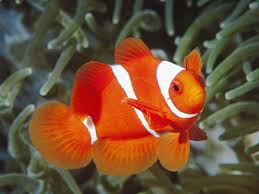
\includegraphics[width=0.95\textwidth]{nemo.jpeg} %% PARA COLOCAR O ARQUIVO DA IMAGEM NO SHARELATEX, CLIQUE NO ÍCONE QUE PARECE UMA FLECHINHA PARA CIMA (ATUALIZAR), CLIQUE EM UPLOAD E PROCURE A IMAGEM EM SEU COMPUTADOR.
\end{figure}


Sinta-se convidado a participar do projeto \abnTeX! Acesse o site do projeto em
\url{http://abntex2.googlecode.com/} (Figura \ref{figura1}). Também fique livre para conhecer,
estudar, alterar e redistribuir o trabalho do \abnTeX, desde que os arquivos
modificados tenham seus nomes alterados e que os créditos sejam dados aos
autores originais, nos termos da ``The \LaTeX\ Project Public
License''\footnote{\url{http://www.latex-project.org/lppl.txt}}.

Encorajamos que sejam realizadas customizações específicas deste exemplo para
universidades e outras instituições --- como capas, folhas de rosto, etc.
Porém, recomendamos que ao invés de se alterar diretamente os arquivos do
\abnTeX, distribua-se arquivos com as respectivas customizações.
Isso permite que futuras versões do \abnTeX~não se tornem automaticamente
incompatíveis com as customizações promovidas. Consulte
\citeonline{abntex2-wiki-como-customizar} par mais informações.

Este documento deve ser utilizado como complemento dos manuais do \abnTeX\ 
\cite{abntex2classe,abntex2cite,abntex2cite-alf} e da classe \textsf{memoir}
\cite{memoir}. 

Equipe \abnTeX 

Lauro César Araujo


% ---
% Capitulo de revisão de literatura
% ---
\chapter{Lorem ipsum dolor sit amet}

% --- Seção dentro do capítulo
\section{Aliquam vestibulum fringilla lorem}
% ---

\lipsum[1]  %% COMANDO QUE COLOCA TEXTO AUTOMÁTICO, SUBSTITUA POR SEU PRÓPRIO TEXTO

\lipsum[2-3]



% ---
% Conclusão
% ---
\chapter*[Conclusão]{Conclusão}
\addcontentsline{toc}{chapter}{Conclusão}

\lipsum[31-33]


% ----------------------------------------------------------
% ELEMENTOS PÓS-TEXTUAIS
% ----------------------------------------------------------
\postextual


% ----------------------------------------------------------
% Referências bibliográficas
% ----------------------------------------------------------
\bibliography{abntex2-modelo-references} %% REFERENCIA AO ARQUIVO abntex2-modelo-references.bib

% ----------------------------------------------------------
% Glossário
% ----------------------------------------------------------
%
% Consulte o manual da classe abntex2 para orientações sobre o glossário.
%
%\glossary

% ----------------------------------------------------------
% Apêndices
% ----------------------------------------------------------

% ---
% Inicia os apêndices
% ---
\begin{apendicesenv}

% Imprime uma página indicando o início dos apêndices
\partapendices

% ----------------------------------------------------------
\chapter{Quisque libero justo}
% ----------------------------------------------------------

\lipsum[50]

% ----------------------------------------------------------
\chapter{Nullam elementum urna vel imperdiet sodales elit ipsum pharetra ligula
ac pretium ante justo a nulla curabitur tristique arcu eu metus}
% ----------------------------------------------------------
\lipsum[55-57]

\end{apendicesenv}
% ---


% ----------------------------------------------------------
% Anexos
% ----------------------------------------------------------

% ---
% Inicia os anexos
% ---
\begin{anexosenv}

% Imprime uma página indicando o início dos anexos
\partanexos

% ---
\chapter{Morbi ultrices rutrum lorem.}
% ---
\lipsum[30]

% ---
\chapter{Cras non urna sed feugiat cum sociis natoque penatibus et magnis dis
parturient montes nascetur ridiculus mus}
% ---

\lipsum[31]

% ---
\chapter{Fusce facilisis lacinia dui}
% ---

\lipsum[32]

\end{anexosenv}

%---------------------------------------------------------------------
% INDICE REMISSIVO
%---------------------------------------------------------------------

\printindex

%---------------------------------------------------------------------
% Formulário de Identificação (opcional)
%---------------------------------------------------------------------
\chapter*[Formulário de Identificação]{Formulário de Identificação}
\addcontentsline{toc}{chapter}{Exemplo de Formulário de Identificação}
\label{formulado-identificacao}

Exemplo de Formulário de Identificação, compatível com o Anexo A (informativo)
da ABNT NBR 10719:2011. Este formulário não é um anexo. Conforme definido na
norma, ele é o último elemento pós-textual e opcional do relatório.

\bigskip

\begin{tabular}{|p{9cm}|p{5cm}|} %% EXEMPLO DE TABELA MAIS COMPLEXA
\hline
\multicolumn{2}{|c|}{\textbf{\large Dados do Relatório Técnico e/ou científico}}\\
\hline
\multirow{4}{10cm}[24pt]{Título e subtítulo}& Classificação de segurança\\
                   & \\
                   \cline{2-2}
                   & No.\\
                   & \\
				
\hline
Tipo de relatório & Data\\
\hline
Título do projeto/programa/plano & No.\\
\hline
\multicolumn{2}{|l|}{Autor(es)} \\
\hline
\multicolumn{2}{|l|}{Instituição executora e endereço completo} \\
\hline
\multicolumn{2}{|l|}{Instituição patrocinadora e endereço completo} \\
\hline
\multicolumn{2}{|l|}{Resumo}\\[3cm]
\hline
\multicolumn{2}{|l|}{Palavras-chave/descritores}\\
\hline
\multicolumn{2}{|l|}{
Edição \hfill No. de páginas \hfill No. do volume \hfill Nº de classificação \phantom{XXXX}} \\
\hline
\multicolumn{2}{|l|}{
ISSN \hfill \hfill Tiragem \hfill Preço \phantom{XXXXXXXX}} \\
\hline
\multicolumn{2}{|l|}{Distribuidor} \\
\hline
\multicolumn{2}{|l|}{Observações/notas}\\[3cm]
\hline
\end{tabular}

\end{document}
